\documentclass[12pt,a4paper]{article}
\usepackage[utf8]{inputenc}
\usepackage[T1]{fontenc}
\usepackage{amsmath}
\usepackage{textcomp}

\usepackage{geometry}
\geometry{a4paper,left=25mm,right=25mm, top=2cm, bottom=2cm} 

\usepackage{graphicx} %fuer bilder

\usepackage{verbatim}




 \usepackage{mathptmx}
 \usepackage[scaled=.90]{helvet}
 \usepackage{courier}



\usepackage{listings}
\usepackage{color}
 
\definecolor{dkgreen}{rgb}{0,0.6,0}
\definecolor{gray}{rgb}{0.5,0.5,0.5}
\definecolor{mauve}{rgb}{0.58,0,0.82}

\pagestyle{empty}
\lstset{numbers=left,language=C++}
\lstset{showstringspaces=false,
basicstyle=\ttfamily\footnotesize,
breaklines=true,
tabsize=3,
commentstyle=\color{dkgreen},      % comment style
inputencoding={ansinew},
title=\lstname %zeigt titel der datei an
}

\usepackage{pdfpages} % fuer pdfs
\usepackage{hyperref} % fuer url


%keine einrückungen bei absatz
\parindent 0pt

\begin{document}
\title{Übung 03}
\author{Reinhard Penn, Bernhard Selymes}
\date{April 2015}

\normalsize

%Beginn des Dokuments

\newcommand{\Uebung}{BFMSV}
\newcommand{\srcpath}{../../src}
\newcommand{\simpath}{../../sim}

%Angabe
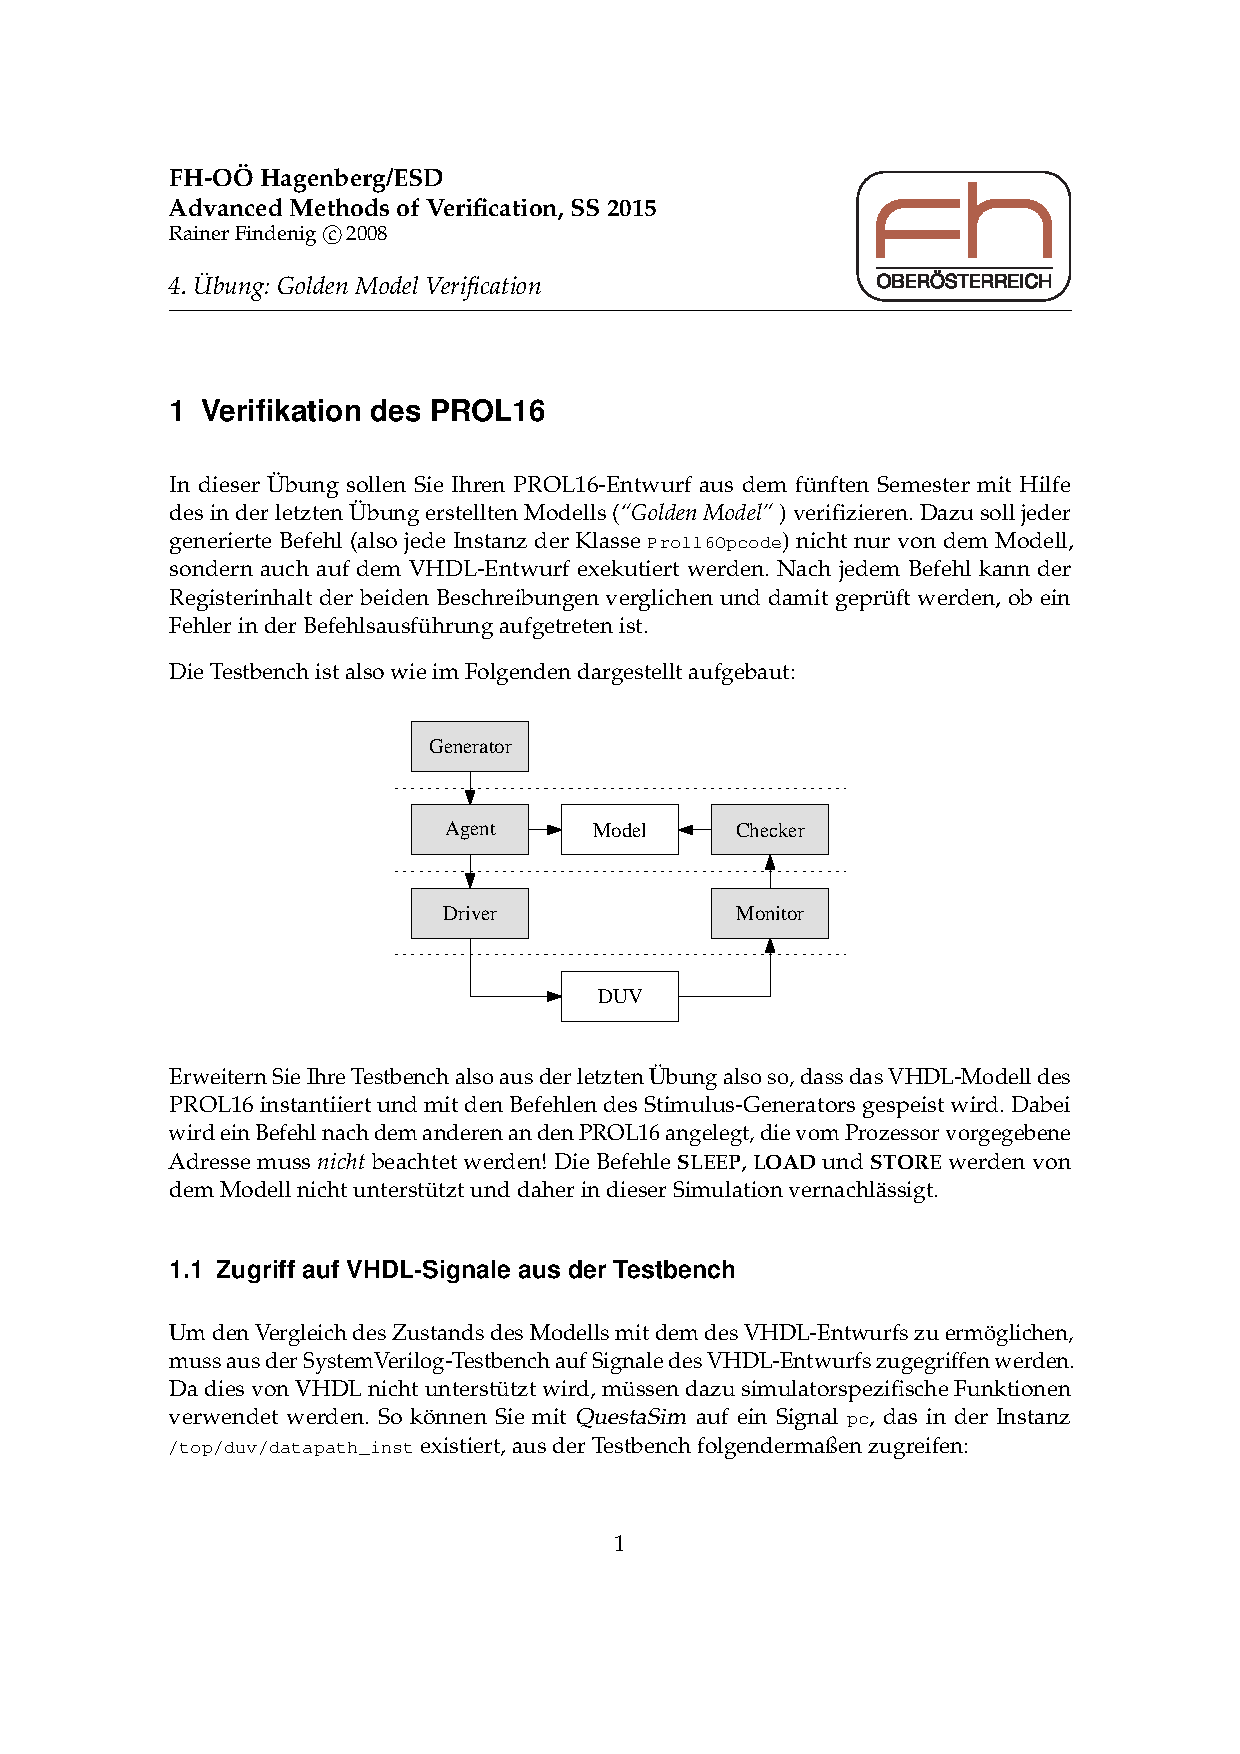
\includepdf[pages=-]{../Angabe.pdf}

\section{Beantwortung der Frage}
Die Funktion hat die Form \texttt{\textdollar signal\_force(<dest\_object>, <value>, <rel\_time>, <force\_type>, <cancel\_period>, <verbose>)}. In der Angabe wurden die Parameter \texttt{<dest\_object>}, \texttt{<value>}, \texttt{<rel\_time>} und \texttt{<force\_type>} verwendet. \\
\texttt{<dest\_object>} ist dabei der Pfad zum Signal, \texttt{<value>} der Wert auf den das Signal gesetzt werden soll, \texttt{<rel\_time>} die relative Zeit wann das Setzen des Signals stattfinden soll und \texttt{<force\_type>} gibt an wie das Signal getrieben werden soll.

\section{Testfälle}
Die Operationen werden auf der CPU, das heißt dem DUV, ausgeführt. Danach werden die Werte vom PC, den Registern und die Flags mit dem Modell des Prol16 verglichen.

Es gibt zwei Möglichkeiten die Register und die Carry Flags zu setzen: Einerseits mithilfe von \texttt{signal\_force} die Signale direkt in der CPU setzen oder andererseits die Register mit \texttt{loadi} zu laden bzw. die Flags mit z.B. Add. 

In den Testfällen wurden die Signale mit \texttt{signal\_force} gesetzt. Das Problem hier ist allerdings dass die Register und Flags dann den Wert behalten und nicht bei der Operation die gerade ausgeführt wird geändert werden. Dies führt dazu, dass die Register und Flags dann beim nächsten Befehl falsch sind.

\section{Source Code}

Der Sourcecode des Prol16 wurde nicht hinzugefügt, da der von der Elearning Plattform verwendet wurde.

\lstinputlisting[language={verilog}]{\srcpath/sv/ifProl16.sv}
\lstinputlisting[language={verilog}]{\srcpath/sv/pkgProl16.sv}
\lstinputlisting[language={verilog}]{\srcpath/sv/Prol16Command.sv}
\lstinputlisting[language={verilog}]{\srcpath/sv/Prol16Opcode.sv}
\lstinputlisting[language={verilog}]{\srcpath/sv/Prol16State.sv}
\lstinputlisting[language={verilog}]{\srcpath/sv/Prol16Model.sv}
\lstinputlisting[language={verilog}]{\srcpath/sv/testProl16Model.sv}
\lstinputlisting[language={verilog}]{\srcpath/sv/top.sv}

\lstinputlisting[language={tcl}]{\simpath/Compile.do}
\lstinputlisting[language={tcl}]{\simpath/Sim.do}

\end{document}
